Solutions of hyperbolic systems are time-reversible as long as shocks
do not form.  This can be used as a computational tool to probe
regularization, following the approach used already in the experiments
of Section \ref{intro}:
\begin{enumerate}
  \item Begin with smooth initial data $q_0$.
  \item Numerically solve \eqref{nel_pde} up to time $T$ to obtain a solution $q_T$.
  \item Reverse the sign of the velocity $u$, to obtain a new solution $q_0^*$.
  \item Numerically solve \eqref{nel_pde} from time $T$ to time $2T$ 
        with initial condition $q_0^*$ to obtain a solution $q_T^*$.
  \item If no shocks formed, the solution $q_T^*$ should match $q_0$, up to
          numerical errors.
\end{enumerate}

%{\bf DK: Replace the following with our Gaussian stress initial condition.
%Replace figures.}

As a demonstration, consider the problem from \cite{leveque2003}, 
which we will call the LY problem
henceforth.  This problem is defined as follows.
We consider the exponential stress relation \eqref{expstress}, and the layered 
medium defined by \eqref{LYmedium} with
$\rho_A=K_A=1 \mbox{  and  } \rho_B=K_B=4$.
An initial pulse is generated by motion of the left boundary:
\begin{align*}
u(0,t) & = \begin{cases} 
  -0.1(1+\cos(\pi(t-10)/10)) & \mbox{for } 0\le t\le 20 \\
  0 & \mbox{for } t>20. \end{cases}
\end{align*}
After a short time, periodic boundary conditions are imposed in
order to observe the long-time behavior of the pulse without using
an excessively large computational domain.
The initial half-cosine pulse evolves into a train
of solitary waves, as shown in Figure \ref{fig:stego}.
%Because of the discontinuous appearance of strain profiles
%(see Figure \ref{fig:strain_train})
%of the solitary waves, they were dubbed 'stegotons'.

\begin{figure}
\centerline{
\subfigure[Initial pulse]{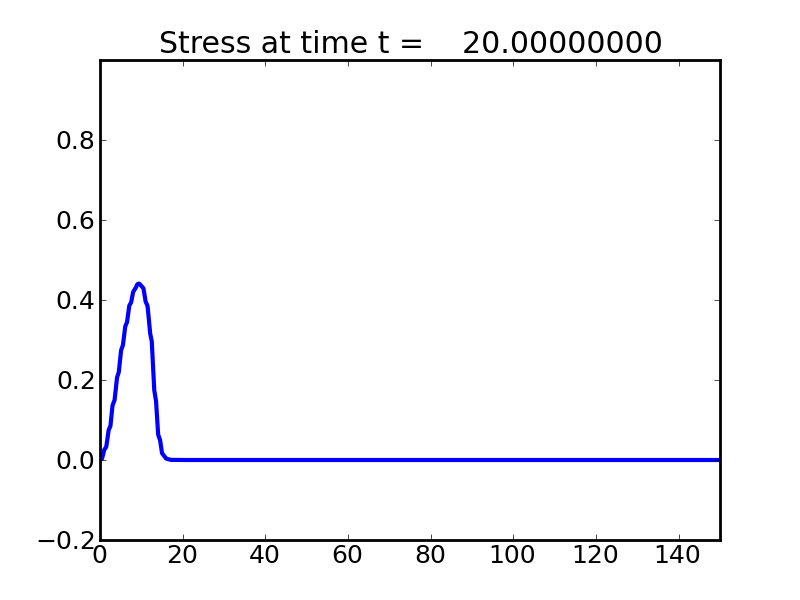
\includegraphics[width=2.5in]{figures/intro_initial_pulse.png}}
%\subfigure[Pulse steepens due to nonlinearity]{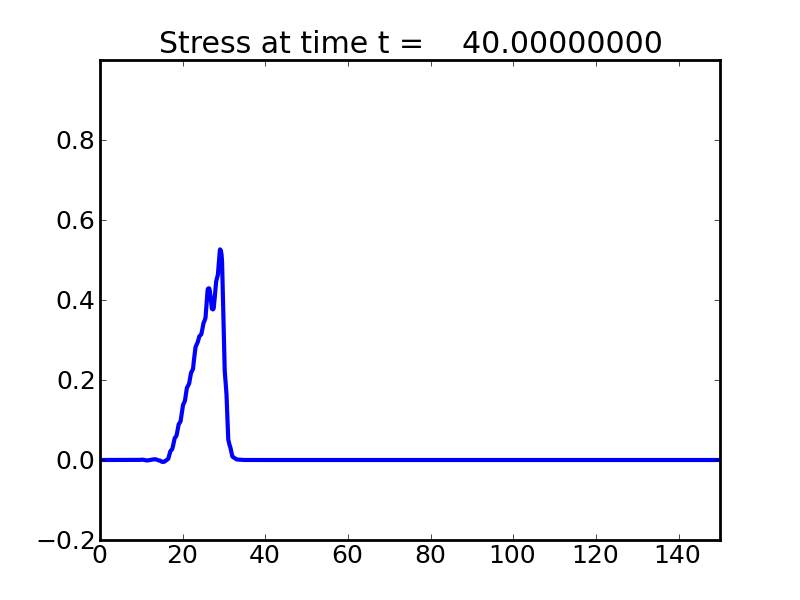
\includegraphics[width=2.5in]{figures/intro_steepens.png}}
\subfigure[Separation into solitary waves]{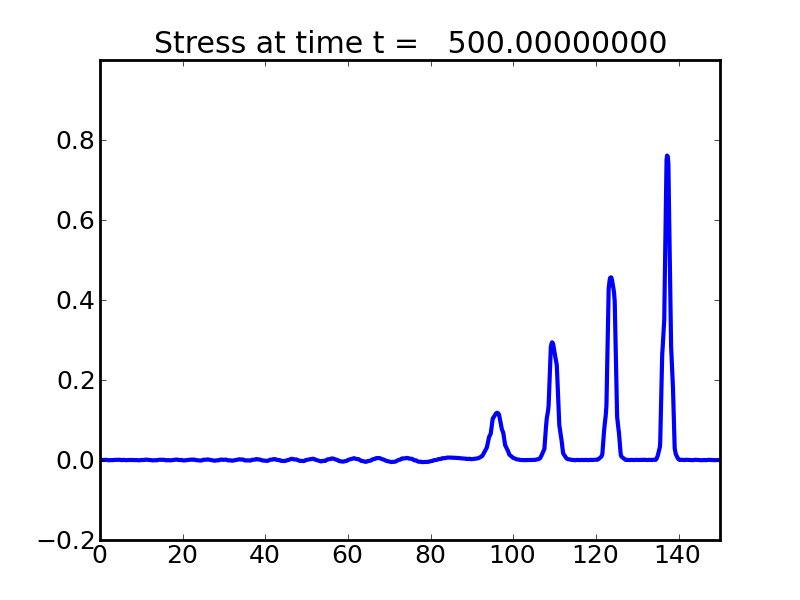
\includegraphics[width=2.5in]{figures/intro_stegotons.png}}}
%\subfigure[Closeup of leading pulse]{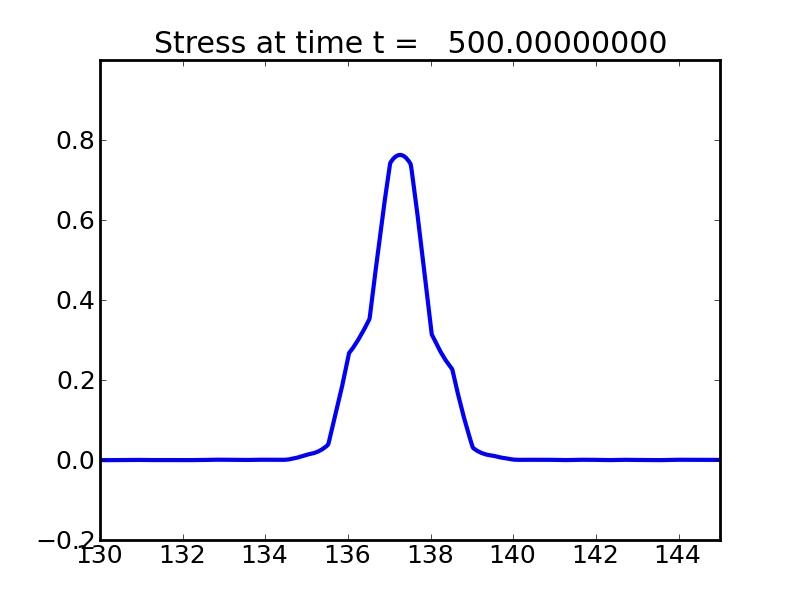
\includegraphics[width=2.5in]{figures/intro_closeup.png}}}
\caption{Evolution of a single pulse into a solitary wave train. \label{fig:stego}}
\end{figure}

%\begin{figure}
%\centerline{
%\includegraphics[width=6in]{figures/stegotons_strain.eps}}
%\caption{Strain profile of solitary wave train.\label{fig:strain_train}}
%\end{figure}

We use the solution to the LY problem at $t=40$ as
initial data, solving up to $T=600$, reversing the velocity, and solving again
up to time $1160$.  
The solutions at these two times,
plotted in \Fig{stego_tr_cp}, appear nearly identical.
Indeed, the maximum pointwise difference of the
initial and final velocities,
\be \label{eq:discrepancy}
E=\|u(x,1160)-u(x,40)\|_\infty,
\ee
which we refer to as the {\em discrepancy}, is quite small.
In \Fig{stego_tr_sc} we plot the 
solution obtained using the SharpClaw software \cite{ketcheson2006} on a grid with 24 cells
per layer.  The $t=1160$ solution (blue squares) is in excellent agreement
with the $t=40$ solution (black line).  
For comparison we also show a solution obtained using Clawpack
on the same grid (24 cells per
layer), in \Fig{stego_tr_cp}.  Clawpack uses second order accurate methods
with limiters, and gives a less accurate 
(but also less computationally expensive) solution on the same grid.
%The SharpClaw runs used the 10-stage, 4th-order Runge-Kutta method of
%\cite{ketcheson2008} with a CFL number of $2.45$, no characteristic
%decomposition, and 5th-order WENO reconstruction.

\begin{figure}
\centerline{
\subfigure[SharpClaw\label{fig:stego_tr_sc}]{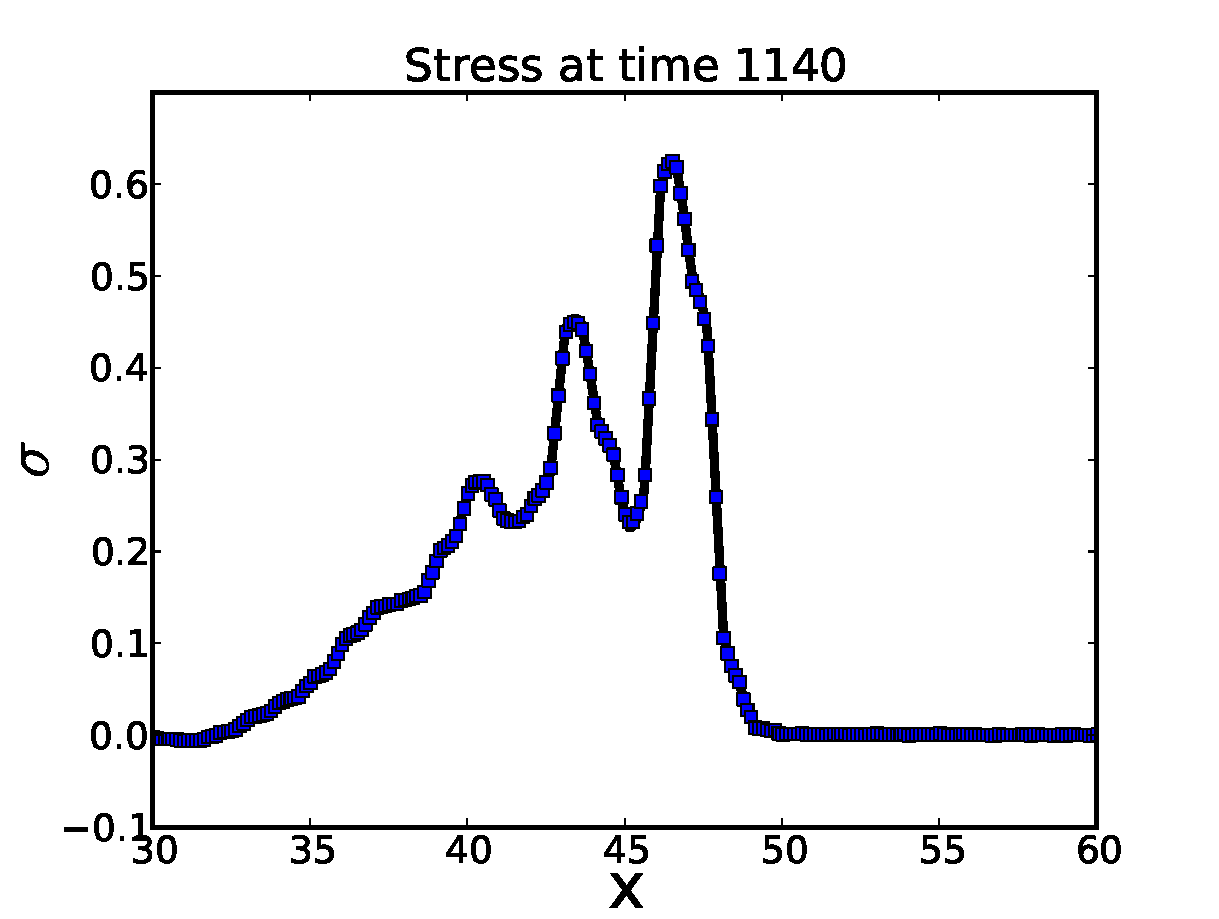
\includegraphics[width=3in]{figures/tr_Z4_sharpclaw.pdf}}
\subfigure[Clawpack\label{fig:stego_tr_cp}]{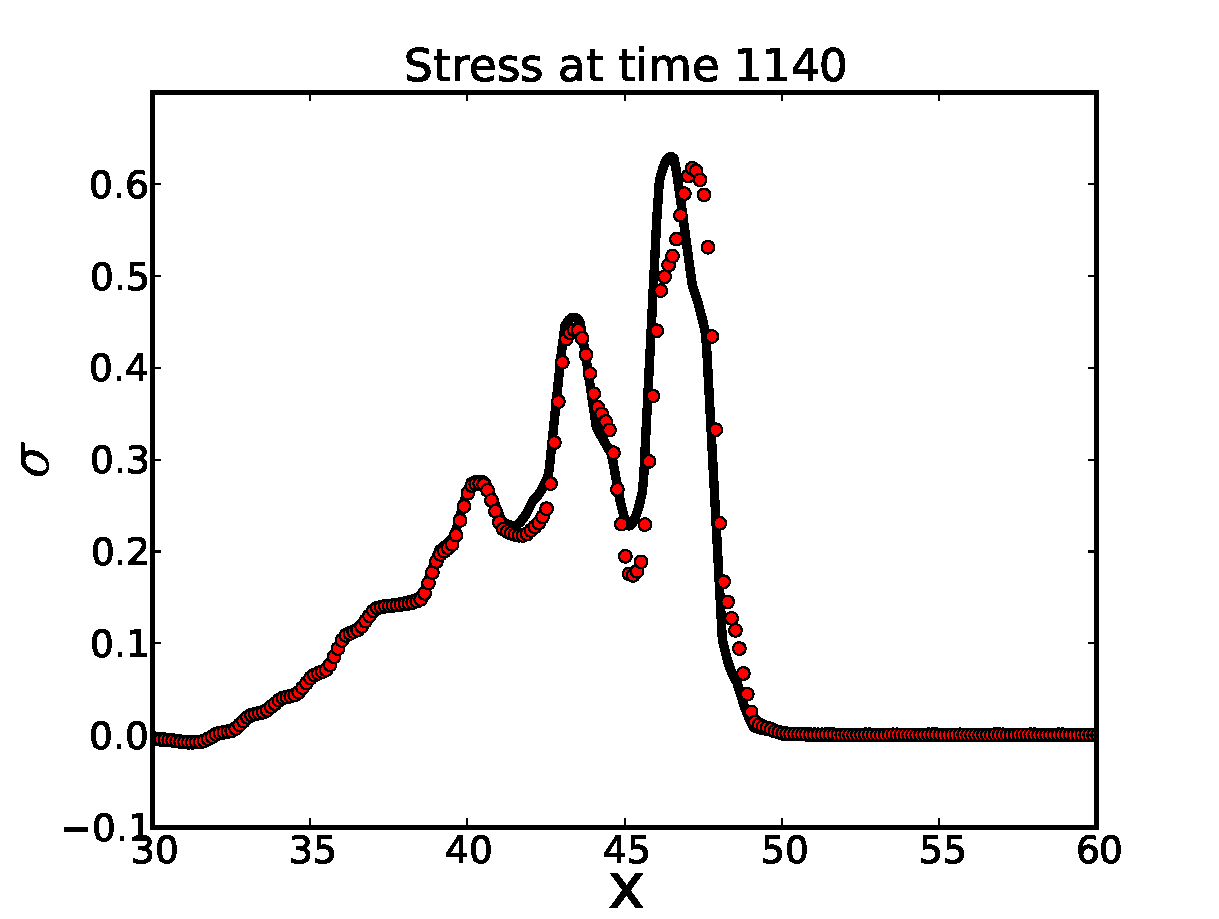
\includegraphics[width=3in]{figures/tr_Z4_clawpack.pdf}}}
\caption[Comparison of forward solution and time-reversed solution 
stegotons.]{Comparison of forward solution (black line) and 
time-reversed solution (symbols).\label{fig:stego_tr}}
\end{figure}

In general the maximum error $E$ is small; We would like to verify 
that the difference between 
initial and final solutions is purely due to numerical errors, and not
due to the formation of (time-irreversible) shocks.  We thus consider
the rate at which $E$ decreases as the grid is refined, using the two 
different numerical methods.
Table \ref{tbl:trconv} lists 
the discrepancy $E$ obtained for a range of grids with both Clawpack and SharpClaw.
By using finer grids, both solutions appears to converge to the early time solution.
The convergence rate of the SharpClaw scheme fluctuates considerably, and
ongoing work is aimed at understanding this.


\begin{table} \centering
\begin{tabular}{r|cc|cc} \hline
& \multicolumn{2}{c}{Clawpack} & \multicolumn{2}{c}{SharpClaw} \\
N & $E$ & Rate & $E$ & Rate \\ \hline
12 & $4.36 \times 10^{-1}$ & -    &  $5.89 \times 10^{-1}$ & -    \\
24 & $8.15 \times 10^{-2}$ & 2.42 &  $8.14 \times 10^{-3}$ & 6.18 \\
48 & $1.54 \times 10^{-2}$ & 2.40 &  $9.81 \times 10^{-4}$ & 3.05 \\
96 & $3.29 \times 10^{-3}$ & 2.23 &  $3.72 \times 10^{-4}$ & 1.40 \\ 
192& $7.41 \times 10^{-4}$ & 2.15 &  $7.86 \times 10^{-5}$ & 2.24 \\ 
%384& $1.85 \times 10^{-4}$ & 2.00\\ 
%768& $5.25 \times 10^{-5}$ & 1.82 \\ 
\hline
\end{tabular}
\caption{Maximum pointwise discrepancy ($E$ defined in \ref{eq:discrepancy}) for 
time-reversal test using Clawpack and Sharpclaw.
The quantity $N$ is the number of computational cells per layer of the
medium.\label{tbl:trconv}}
\end{table}


Next we conduct the same test but with a less-strongly varying medium,
taking $\rho_B=K_B=Z_B=2$.
\Fig{stego_ntr} shows the results obtained with SharpClaw using 24 and
48 cells per layer.  Observe the large 
difference between the initial and final solutions.
This seems to indicate that shock formation has occurred in 
this case, leading to a loss of time-reversibility.
%{\bf should we discuss the importance of impedance contrast before this?
%YES.  Also, add a figure showing the shocks that form in this case.}

\begin{figure} \centering
\subfigure[24 cells per layer]{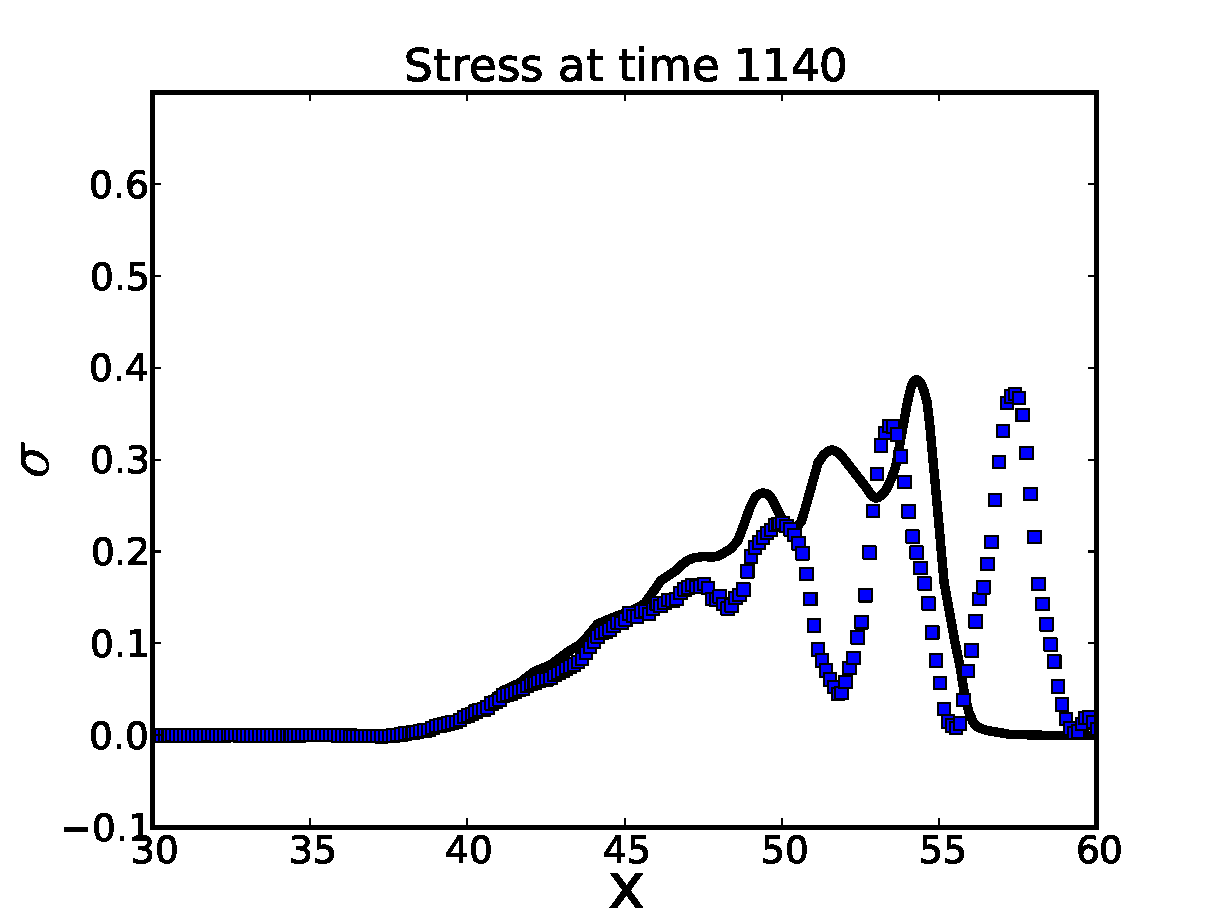
\includegraphics[width=3in]{figures/tr_Z2_sharpclaw_24.pdf}}
\subfigure[48 cells per layer]{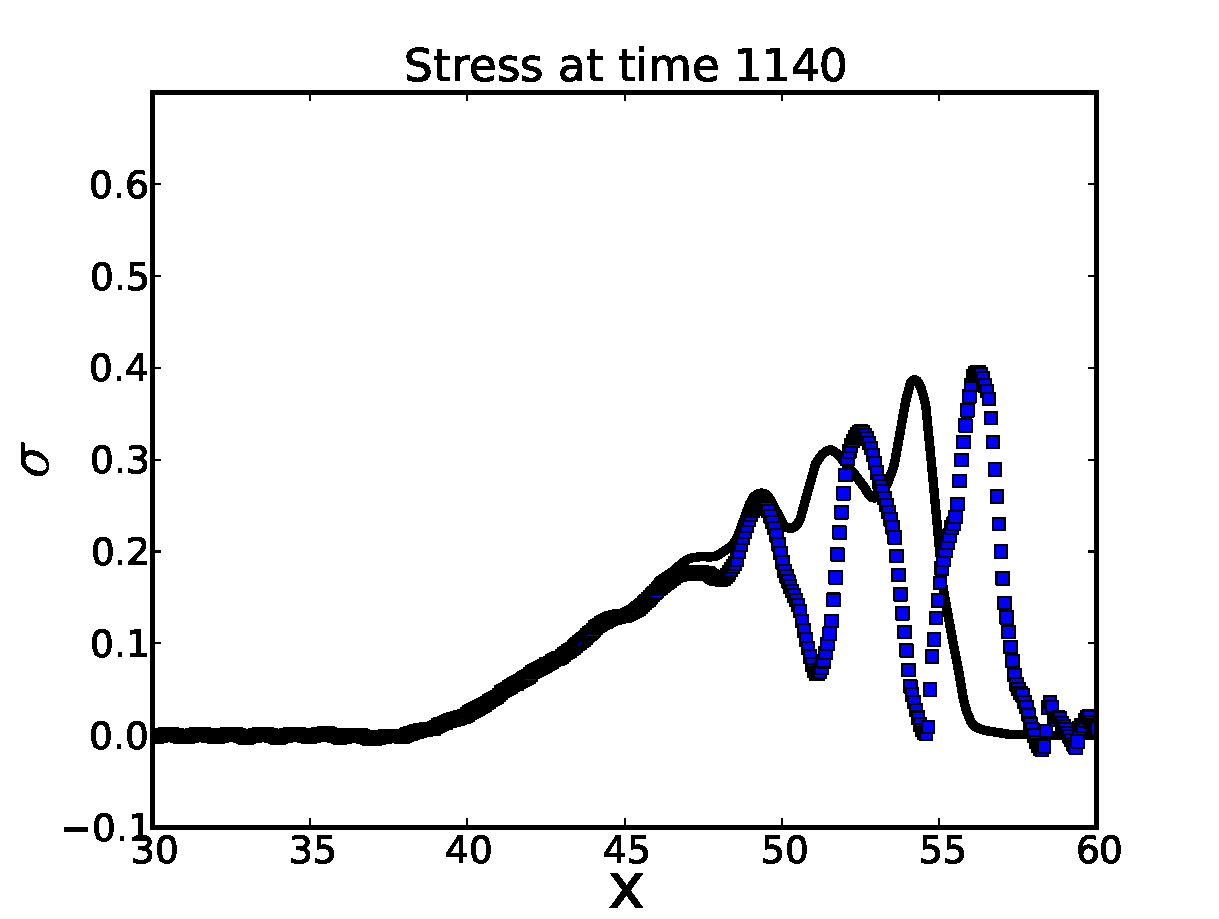
\includegraphics[width=3in]{figures/tr_Z2_sharpclaw_48.pdf}}
\caption{Comparison of forward solution (solid line) and 
time-reversed solution (dotted line) obtained with SharpClaw 
using 24 and 48 cells per layer, for an LY medium
with lower impedance contrast $Z_B=2$.
The solution seems not to be time-reversible.
\label{fig:stego_ntr}}
\end{figure}


%Observe that even the homogenized equations \eqref{} are time-reversible,
%since all terms involving an even number of spatial derivatives 
%vanish for piecewise periodic media \cite{leveque2003}.
%Thus, the resulting equations are invariant under the transformation
%\begin{subequations}
%\begin{align}
%u \to & -u \\
%x \to & -x
%\end{align}
%\end{subequations}
%However, this argument would imply that waves that obey the 1D elasticity
%equations \eqref{nel_pde} are time-reversible in any piecewise constant 
%medium; as we will see, this is not the case.  


